\documentclass[tikz]{standalone}
\usepackage{fontspec} % BUILD WITH XELATEX
\setmainfont{Arial}

\usepackage{tikz}
\usetikzlibrary{positioning}
\usetikzlibrary{calc}
\usetikzlibrary{arrows.meta}
\usepackage{pgfmath}
\usepackage{amsmath}

% \tikzset{
%   treenode/.style = {align=center, inner sep=2pt, text centered,
%     font=\sffamily},
%   arn_n/.style = {treenode, align=left, draw=white}% arbre rouge noir, noeud noir
% }

\begin{document}

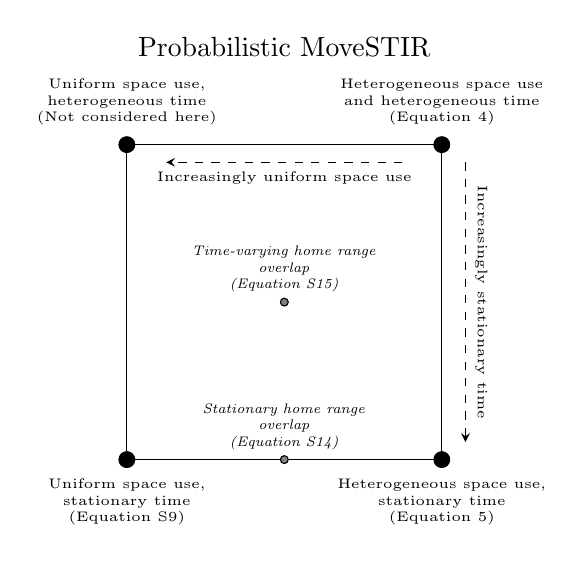
\begin{tikzpicture}
    
    \pgfmathsetmacro{\scale}{4}
    \pgfmathsetmacro{\rad}{.1}

    % Draw corners
    \draw[fill] (0, 0) circle  [radius=\rad cm] node (ur) {};
    \draw[fill] (0, -1*\scale) circle  [radius=\rad cm] node (lr) {};
    \draw[fill] (-1*\scale, 0) circle  [radius=\rad cm] node (ul) {};
    \draw[fill] (-1*\scale, -1*\scale) circle  [radius=\rad cm] node (ll) {};

    % Draw edges
    \draw[-] (ur.center)--(lr.center);
    \draw[-] (ur.center)--(ul.center);
    \draw[-] (ul.center)--(ll.center);
    \draw[-] (ll.center)--(lr.center);

    \node[at=(ur.north), above, font=\tiny, align=center] {Heterogeneous space use\\and heterogeneous time \\ (Equation 4)};
    \node[at=(lr.south), below, font=\tiny, align=center] {Heterogeneous space use,\\ stationary time \\ (Equation 5)};
    \node[at=(ll.south), below, font=\tiny, align=center] {Uniform space use,\\stationary time \\ (Equation S9)};
    \node[at=(ul.north), above, font=\tiny, align=center] {Uniform space use,\\heterogeneous time \\ (Not considered here)};


    \draw[-stealth, dashed] ($(ur.south) + (-0.5, -0.1)$)--($(ul.south) + (0.5, -0.1)$) node[midway, below, font=\tiny, align=center] {Increasingly uniform space use};

    \draw[-stealth, dashed] ($(ur.south) + (0.3, -0.1)$)--($(lr.north) + (0.3, 0.1)$) node[midway, above, font=\tiny, align=center, rotate=-90] {Increasingly stationary time};


    \draw[fill=gray] (-1*\scale*0.5, -1*\scale) circle  [radius=\rad*0.5 cm] node[above, font=\tiny, align=center] (hro) {\emph{Stationary home range}\\\emph{overlap} \\ \emph{(Equation S14)}};

    \draw[fill=gray] (-1*\scale*0.5, -1*\scale*0.5) circle  [radius=\rad*0.5 cm] node[above, font=\tiny, align=center] (hro) {\emph{Time-varying home range}\\\emph{overlap} \\ \emph{(Equation S15)}};

    % \draw[fill=gray] (-1*\scale*0, -1*\scale*0.5) circle  [radius=\rad*0.5 cm] node[above, left, font=\tiny, align=center] (hro) {\emph{Time-varying UD}\\\emph{overlap} \\ \emph{(Equation SX)}};

    \node[above] at (-1*\scale*0.5, 0.25*\scale*1) {Probabilistic MoveSTIR};

\end{tikzpicture}

\end{document}

